\documentclass[paper=letter, fontsize=11pt]{scrartcl} % Letter paper and 11pt font size

\usepackage{amstext, amsmath, amssymb, graphicx}
\usepackage[T1]{fontenc} % Use 8-bit encoding that has 256 glyphs
\usepackage[english]{babel} % English language/hyphenation
\usepackage{amsmath,amsfonts,amsthm} % Math packages

\usepackage{fancyhdr} % Custom headers and footers
\pagestyle{fancyplain} % Makes all pages in the document conform to the custom headers and footers
\fancyhead{} % No page header
\fancyfoot[L]{} % Empty left footer
\fancyfoot[C]{} % Empty center footer
\fancyfoot[R]{\thepage} % Page numbering for right footer
\renewcommand{\headrulewidth}{0pt} % Remove header underlines
\renewcommand{\footrulewidth}{0pt} % Remove footer underlines
\setlength{\headheight}{13.6pt} % Customize the height of the header
\setlength\parindent{0pt} % Removes all indentation from paragraphs

%----------------------------------------------------------------------------------------
%	TITLE SECTION
%----------------------------------------------------------------------------------------

\newcommand{\horrule}[1]{\rule{\linewidth}{#1}} % Create horizontal rule command with 1 argument of height

\title{	
\normalfont \normalsize 
\textsc{San Francisco State University} \\ [25pt]
\horrule{0.5pt} \\[0.4cm] % Thin top horizontal rule
\huge MATH 490 Assignment 2  \\ % The assignment title
\horrule{2pt} \\[0.5cm] % Thick bottom horizontal rule
}

\author{Omar Sandoval}

\date{\normalsize\today}

\begin{document}

\maketitle

%----------------------------------------------------------------------------------------
%	PROBLEM 2.2
%----------------------------------------------------------------------------------------
\textbf{2.2} For diagnostic testing, let $X$ = \textit{true} status (1 = disease, 2 = no disease)
and $Y$ = diagnosis (1 = positive, 2 = negative),Let $\pi_i = P(Y = 1|x = i)$, $i = 1, 2$. \\

\textbf{a.} Explain why sensitivity = $\pi_1$ and specificity = $1 - \pi_2$.
\begin{align*}
	&\text{Sensitivity is equal to } P(Y = 1 | X = 1) = \pi_1. \\
	&\text{Specificity is equal to } P(Y = 2 | X = 2) = 1 - P(Y = 1 | X = 2) = 1 - \pi_2.
\end{align*}

\textbf{b.} Let $\gamma$ denote the probability that a subject has the disease. Given
that the diagnosis is positive, use Baye's theorem to show that the probability a
subject truly has the disease is;
\begin{align*}
	\pi_1\gamma/[\pi_1\gamma + \pi_2(1 - \gamma)]
\end{align*} \\
$\gamma = P(X = 1)$ \\

To find the probability a subject truly has the disease, $X$ must equal 1 given that $Y$ equals 1. \\
So, \\
$P(X = 1 | Y = 1) = \dfrac{P(Y = 1 | X = 1)\gamma}{P(Y = 1 | X = 1)\gamma + P(Y = 1 | X = 2)\gamma}
= \dfrac{\pi_1\gamma}{\pi_1\gamma + \pi_2(1 - \gamma)}$ \\

\textbf{c.} For mammograms for detecting breast cancer, suppose $\gamma$ = 0.01, sensitivity = 0.86,
and specificity = 0.88. Given a positive test result, find the probability that the woman truly
has breast cancer. \\
\\ 
$\dfrac{.86(.01)}{.86(.01) + .12(.99) = .0675}$ probability. \\
\\

\textbf{d.} To better understand the answer in (c), find the joint probabilities for the $2 \times 2$
cross classification of $X$ and $Y$. Discuss their relative sizes in the two cells that refer to 
a positive test result. \\
\\
\begin{table}[h]
\begin{tabular}{l|l|l|l|l}
     &            & +      & -      & Total \\
True & disease    & 0.0086 & 0.0014 & 0.01  \\
     & no disease & 0.1188 & 0.8712 & 0.99     
\end{tabular}
\end{table}

Almost all of the subjects do not have breast cancer. A very high proportion is contained in the 
"no disease" category compared to the "disease" category. \\

%----------------------------------------------------------------------------------------
%	PROBLEM 2.4
%----------------------------------------------------------------------------------------
\textbf{2.4} A newspaper article preceding the 1994 World Cup semifinal match between Italy and 
Bulgaria stated that "Italy is favored 10-11 to beat Bulgaria, which is rated at 10-3 to reach 
the final." Suppose this means that the odds that Italy wins are 3/10. Find the probability that
each team wins, and comment. \\
 
The probability that Italy wins is $\dfrac{1.1}{1 + 1.1} = 0.5238.$ \\
The probability that Bulgaria wins is $\dfrac{.3}{1 + .3} = -.2308.$ \\
$.5238 + .2308 = .7546 \not= 1$, therefore, the two odds do not agree with each other. \\

%----------------------------------------------------------------------------------------
%	PROBLEM 2.6
%----------------------------------------------------------------------------------------
\textbf{2.6} In the United States, the estimated annual probability that a women over the age
of 35 dies of lung cancer equals 0.001304 for current smokers and 0.000121 for nonsmokers
[M. Pagano and K. Gauvreau, \textit{Principles of Biostatistics}, Belmont, CA: Duxbury Press (1993), p
. 134]. \\

\textbf{a.} Calculate and interpret the difference of proportions and the relative risk.
Which is more informative for these data? Why? \\

Difference: $0.001304 - 0.000121 = 0.001183$ \\
Relative risk: $0.001304 / 0.000121 = 10.7769$ \\
The difference of proportions only tells us that the difference between proportions of female smokers/non-smokers
who die is only .12 percent.
Relative risk tells us that a woman over 35 dying of lung cancer is 10.78 times higher for smokers than nonsmokers.
Relative risk is more telling of the data since the difference makes it seem like there is very little
association between the two. \\

\textbf{b.} Calculate and interpret the odds ratio. Explain why the relative risk and odds ratio
take similar values. \\

Odds Ratio: $\theta = \dfrac{.001304/.998696}{.000121/.999879} = 10.79$ \\
The odds of a smoking woman over 35 dying of lung cancer are 10.79 times higher than a nonsmoking woman
over 35 dying of lung cancer. The relative risk and odds ratio take close values when the proportion in
the first category is close to zero. In this case, that was "dying of lung cancer". \\


%----------------------------------------------------------------------------------------
%	PROBLEM 2.12
%----------------------------------------------------------------------------------------
\textbf{2.12} A statistical analysis that combines information from several studies is
called a \textit{meta analysis}. A meta analysis compared aspirin with placebo on
incidence of heart attack and of stroke, separately for men and for women
(\textit{J. Am. Med. Assoc.}, \textbf{295}: 306-313, 2006). For the Women's Health Study,
heart attacks were reported for 198 of 19,934 taking aspirin and for 193 of
19,942 taking placebo. \\

\textbf{a.} Construct the $2 \times 2$ table that cross classifies the treatment (aspirin,
placebo) with whether a heart attack was reported (yes, no). \\

\begin{table}[h]
\begin{tabular}{l|l|l|l}
Group   & Yes & No     & Total  \\
Placebo & 193 & 19,749 & 19,942 \\
Aspirin & 198 & 19,736 & 19,934
\end{tabular}
\end{table}

\textbf{b.} Estimate the odds ratio. Interpret. \\
Odds Ratio: $\theta = 0.9839$. Sample odds for a heart attack are a little bit less for the placebo group.

\textbf{c.} Find a 95 percent confidence interval for the population odds ratio for women.
Interpret.(As of 2006, results suggested that for women, aspirin was helpful 
for reducing risk of stroke but not necessarily risk of heart attack.) \\

CI for odds ratio for women: $(0.8061, 1,2008)$.
It can be argued that there is no effect.
\\

%----------------------------------------------------------------------------------------
%	PROBLEM 2.16
%----------------------------------------------------------------------------------------
\textbf{2.16} Table 2.12 comes from one of the first studies of the link between lung cancer
and smoking, by Richard Doll and A. Bradford Hill. In 20 hospitals in London,
UK, patients admitted with lung cancer in the previous year were queried
about their smoking behavior. For each patient admitted, researchers studied
the smoking behavior of a noncancer control patient at the same hospital of the same sex
and within the same 5-year grouping on age. A smoker was defined as a person who had smoked 
at least one cigarette a day for at least a year. \\

\textbf{a.} Identify the response variable and the explanatory variable. \\

The response variable is whether the patient has smoked or not. The explanatory
variable is the lung cancer.

\textbf{b.} Identify the type of study this was. \\

This study was a case-control study.

\textbf{c.} Can you use these date to compare smokers with nonsmokers in terms of the proportion
who suffered lung cancer? Why or why not? \\
 
Patients in control group may not have lung cancer, but that does not mean they do not suffer from
other health conditions. These conditions could have an impact on their health and whether they have 
lung cancer or not. In this case, a comparison would not show whether there is a relationship between
a patients smoking habits and their lung cancer status.
 
 
\textbf{d.} Summarize the association, and explain how to interpret it. \\

We can use the odds ratio to form a conclusion about the data. \\
Odds Ratio: $\theta = \dfrac{688(59)}{650(21)} = 2.9738$. The odds of having lung cancer are 2.9 times higher
for someone who smokes compared to someone who doesn't smoke.

\begin{center}
	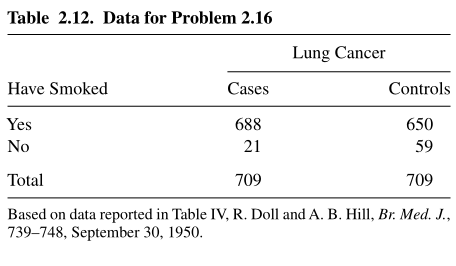
\includegraphics[scale=0.75]{table216.png}
\end{center}


%----------------------------------------------------------------------------------------
%	PROBLEM 2.18
%----------------------------------------------------------------------------------------
\textbf{2.18 DO NOT DO.}


\end{document}
